\section{Tipos de M\'aser}
\label{tipos}

Existen tres tipos principales de m\'aser: los de rayo at\'omico, los de gas y los de estado s\'olido. En esta secci\'on hablaremos brevemente de cada uno de estos tres tipos, aunque sin entrar en detalles sobre su funcionamiento a nivel at\'omico.

\subsection{M\'aser de rayo at\'omico}

Los principales m\'aseres de rayo at\'omico son los de hidr\'ogeno y los de amon\'iaco.

\subsubsection{M\'aser de amon\'iaco}

El primer m\'aser, construido por Charles H. Townes y su equipo en la Universidad de Columbia en 1953, utilizaba un haz de mol\'eculas de \textbf{amon\'iaco} para producir la amplificaci\'on de microondas a la frecuencia de 24 GigaHerzios. En la Figura \ref{fig:maser_amoniaco} se muestra la estructura de este tipo de m\'aser \cite{AmoniaMaser}.

\begin{figure}[ht!]
 \centering
 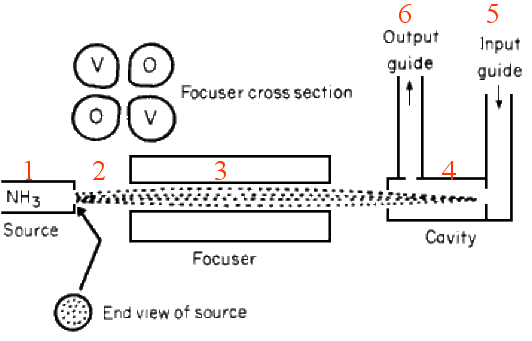
\includegraphics[width=0.6\textwidth]{./Utils/maser_amoniaco.png}
 % maser_hidrogeno.png: 200x375 pixel, 72dpi, 7.06x13.23 cm, bb=0 0 200 375
 \caption{Estructura de un m\'aser de amon\'iaco}
 \label{fig:maser_amoniaco}
\end{figure}

En el m\'aser de amon\'iaco, el gas se calienta primero y las moleculas excitadas se hacen pasar a trav\'es de un campo el\'ectrico no uniforme, de forma que se \textit{recogen} \cite{ElectroAplicado}. Despu\'es las mol\'eculas excitadas pasan a trav\'es de una cavidad, donde ceden su energ\'ia y pasan a su estado de menor energ\'ia. La cesi\'on de energ\'ia se lleva a cabo a trav\'es de una emisi\'on a cierta frecuencia, a la cual la cavidad est\'a sintonizada. Esta frecuencia viene dada por la ley de Planck, y es exactamente 23,87 GHz.



\subsubsection{M\'aser de hidr\'ogeno}
\label{tipo:hidrogeno}

Despu\'es de la creaci\'on del primer m\'aser de amon\'iaco, en 1960 Ramsey y sus colegas de Harvard desarrollaron un máser que funcionaba con hidrógeno y podía utilizarse como un reloj atómico de extremada precisión.

Un m\'aser de hidr\'ogeno, tambi\'en conocido como est\'andar de frecuencia de hidr\'ogeno, es un tipo de m\'aser espec\'ifico que aprovecha las propiedades intr\'insecas del hidr\'ogeno para proporcionar una referencia en frecuencia de precisi\'on. La frecuencia de oscilaci\'on del \'atomo de hidr\'ogeno (su frecuencia de resonancia) es de 1420 MHz.

\begin{figure}[ht!]
 \centering
 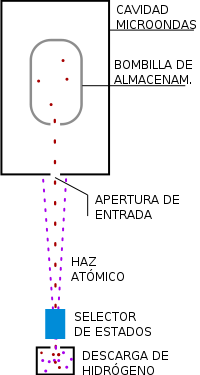
\includegraphics[width=0.33\textwidth]{./Utils/maser_hidrogeno.png}
 % maser_hidrogeno.png: 200x375 pixel, 72dpi, 7.06x13.23 cm, bb=0 0 200 375
 \caption{Estructura de un maser de hidrógeno}
 \label{fig:maser_hidrogeno}
\end{figure}

Los m\'aseres de hidr\'ogeno son dispositivos muy complejos y muy caros. De hecho, es el más costoso de los estándares en frecuencia, y los pocos que existen están en laboratorios internacionales de calibración.

Existen dos tipos de m\'aseres de hidr\'ogeno: activos y pasivos. El m\'aser activo oscila espont\'aneamente y un oscilador de cuarzo se engancha en fase a esta frecuencia de oscilaci\'on. El m\'aser pasivo opera enganchando en frecuencia un oscilador de cuarzo. 



En los dos tipos de m\'aser un peque\~no bote de almacenamiento de hidr\'ogeno molecular (pares de \'atomos de hidr\'ogeno unidos) suelta una cantidad controlada de gas en una cavidad de descarga (ver Figura \ref{fig:maser_hidrogeno}). En esta cavidad las mol\'eculas se separan en \'atomos de hidr\'ogeno individuales mediante un arco. Este hidr\'ogeno at\'omico atraviesa un selector de estado magn\'etico, donde se selecciona el estado deseado antes de hacerlos pasar a la \textit{bombilla} de almacenamiento. Esta bombilla suele tener 20 cm de alto y 10 cm de di\'ametro, y suele estar hecha de cuarzo y revestida de tefl\'on por dentro. Este revestimiento ralentiza la recombinaci\'on de los \'atomos de hidr\'ogeno en mol\'eculas de hidr\'ogeno. 

La bombilla de almacenamiento est\'a situada dentro de una cavidad microondas, que est\'a sintonizada a la frecuencia de resonancia de los \'atomos, 1420 MHz.

Como se ha mencionado antes, en el m\'aser activo la cavidad oscila por s\'i misma. Esto requiere una mayor densidad de \'atomos de hidr\'ogeno y un factor de calidad mayor para la cavidad. El m\'aser activo es m\'as complejo y m\'as caro, pero tiene una mejor estabilidad en frecuencia a largo plazo.

En el m\'aser pasivo, la cavidad se alimenta con una frecuencia externa de 1420 MHz. Esto permite usar una densidad de \'atomos de hidr\'ogeno menor y tambi\'en un menor factor de calidad en la cavidad, lo que reduce el coste.

Ambos tipos de m\'aser poseen mejor estabilidad a corto plazo que los osciladores de cesio. Sin embargo, ya que el comportamiento de un m\'aser de hidr\'ogeno depende de numerosos factores ambientales, posee una incertidumbre en frecuencia mayor que la de los osciladores de cesio, por lo que son peores para medir largos espacios de tiempo.

\subsection{M\'aseres de gas}

El \textbf{m\'aser de rubidio} \cite{rubidium} es un ejemplo de m\'aser de gas utilizado de forma habitual. Al igual que el m\'aser de hidr\'ogeno, sirve como reloj at\'omico. El m\'aser de rubidio es menos preciso, pero tambi\'en menos costoso.

La frecuencia de resonancia del rubidio es 6 834 682 614 Hz, es decir, unos 6,834 GHz. 

El primer est\'andar de frecuencia de rubidio surgi\'o como resultado del trabajo de Carpenter y Arditi en 1960. A\~nos m\'as tarde, en 1964, Davidovits construy\'o el primer m\'aser de rubidio operativo.

El m\'aser de rubidio, al igual que el de hidr\'ogeno, puede funcionar en modo activo o pasivo. El modo pasivo es el m\'as \'util, ya que con un tama\~no menor mantiene una estabilidad en frecuencia excelente. Este dispositivo tiene numerosas aplicaciones en el campo de las comunicaciones, en el espacio y en navegaci\'on, y tiene una estructura similar al m\'aser de hidr\'ogeno.

\subsection{M\'aseres de estado s\'olido}

Los m\'aseres de estado s\'olido \cite{historiaFisica} se basan en hacer transmisiones cu\'anticas en \'atomos con tres niveles de energ\'ia en los cuales el nivel intermedio es metaestable.

La exitosa familia de los\textbf{ m\'aseres de rub\'i} fue iniciada por Chihiro Kukuchi y sus colegas en la Universidad de Michigan. Por su baja temperatura de ruido, los m\'aseres de estado s\'olido encontraron un uso temprano en los radiotelescopios y en antenas de microondas.

\subsection{M\'aseres astron\'omicos}

Adem\'as de los m\'aseres creados por el hombre, existen \textbf{m\'aseres naturale}s presentes en el universo. Estos son los m\'aseres astron\'omicos, que se utilizan para aprender m\'as sobre la composici\'on y constituci\'on del universo. 

Para que en el espacio se produzca una emisi\'on m\'aser \cite{maserEspacio} deben darse como m\'inimo dos condiciones: En primer lugar, tiene que haber la suficiente cantidad de gas para que sus mol\'eculas puedan amplificar la radiaci\'on. En segundo lugar, debe existir una importante fuente de energ\'ia que produzca la inversi\'on de poblaci\'on, es decir, que suba a las mol\'eculas a su nivel de alta energ\'ia. Estas condiciones se dan en diferentes ambientes: regiones de formaci\'on estelar, cometas, atm\'osferas planetarias, estrellas en sus \'ultimas fases de vida e incluso cerca de los agujeros negros centrales de algunas galaxias.

El motivo por el que se produce el efecto m\'aser en estas zonas es que el hidr\'ogeno gaseoso, componente fundamental de la materia interestelar, es especialmente densa en estas regiones. Adem\'as de hidr\'ogeno en la materia interestelar hay otras mol\'eculas, y algunas de ellas act\'uan como amplificadores de radiaci\'on y producen la intensa emisi\'on m\'aser. Los máseres más utilizados en Astronomía son los producidos por el radical hidroxilo, el monóxido de silicio, el metanol y el agua.

La Figura \ref{fig:maser_astronomico} muestra la emisi\'on m\'aser de una estrella en formaci\'on \cite{fotoMaser}. Los c\'irculos blancos representan zonas de emisi\'on m\'aser de la mol\'ecula de agua, que trazan un disco de gas en el que podr\'ia estar form\'andose un nuevo sistema planetario. En color se muestra la emisi\'on en radio de un chorro de material expulsado en direcci\'on perpendicular al disco.

\begin{figure}[ht!]
 \centering
 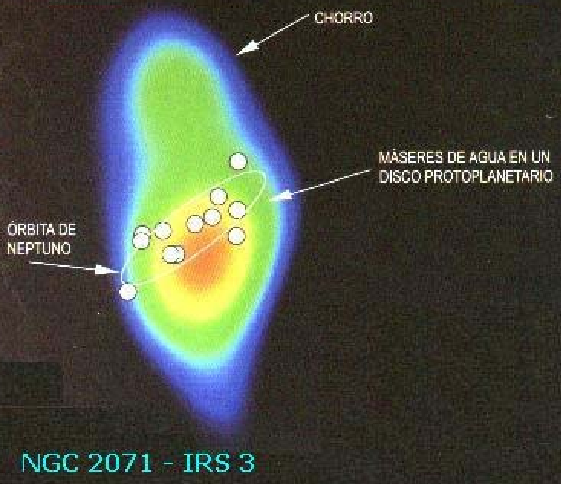
\includegraphics[width=0.6\textwidth]{./Utils/maser_astronomico.png}
 % maser_hidrogeno.png: 200x375 pixel, 72dpi, 7.06x13.23 cm, bb=0 0 200 375
 \caption{Emisi\'on m\'aser de una estrella en formaci\'on}
 \label{fig:maser_astronomico}
\end{figure}
